\documentclass{article}\usepackage{graphicx, color}
%% maxwidth is the original width if it is less than linewidth
%% otherwise use linewidth (to make sure the graphics do not exceed the margin)
\makeatletter
\def\maxwidth{ %
  \ifdim\Gin@nat@width>\linewidth
    \linewidth
  \else
    \Gin@nat@width
  \fi
}
\makeatother

\IfFileExists{upquote.sty}{\usepackage{upquote}}{}
\definecolor{fgcolor}{rgb}{0.2, 0.2, 0.2}
\newcommand{\hlnumber}[1]{\textcolor[rgb]{0,0,0}{#1}}%
\newcommand{\hlfunctioncall}[1]{\textcolor[rgb]{0.501960784313725,0,0.329411764705882}{\textbf{#1}}}%
\newcommand{\hlstring}[1]{\textcolor[rgb]{0.6,0.6,1}{#1}}%
\newcommand{\hlkeyword}[1]{\textcolor[rgb]{0,0,0}{\textbf{#1}}}%
\newcommand{\hlargument}[1]{\textcolor[rgb]{0.690196078431373,0.250980392156863,0.0196078431372549}{#1}}%
\newcommand{\hlcomment}[1]{\textcolor[rgb]{0.180392156862745,0.6,0.341176470588235}{#1}}%
\newcommand{\hlroxygencomment}[1]{\textcolor[rgb]{0.43921568627451,0.47843137254902,0.701960784313725}{#1}}%
\newcommand{\hlformalargs}[1]{\textcolor[rgb]{0.690196078431373,0.250980392156863,0.0196078431372549}{#1}}%
\newcommand{\hleqformalargs}[1]{\textcolor[rgb]{0.690196078431373,0.250980392156863,0.0196078431372549}{#1}}%
\newcommand{\hlassignement}[1]{\textcolor[rgb]{0,0,0}{\textbf{#1}}}%
\newcommand{\hlpackage}[1]{\textcolor[rgb]{0.588235294117647,0.709803921568627,0.145098039215686}{#1}}%
\newcommand{\hlslot}[1]{\textit{#1}}%
\newcommand{\hlsymbol}[1]{\textcolor[rgb]{0,0,0}{#1}}%
\newcommand{\hlprompt}[1]{\textcolor[rgb]{0.2,0.2,0.2}{#1}}%

\usepackage{framed}
\makeatletter
\newenvironment{kframe}{%
 \def\at@end@of@kframe{}%
 \ifinner\ifhmode%
  \def\at@end@of@kframe{\end{minipage}}%
  \begin{minipage}{\columnwidth}%
 \fi\fi%
 \def\FrameCommand##1{\hskip\@totalleftmargin \hskip-\fboxsep
 \colorbox{shadecolor}{##1}\hskip-\fboxsep
     % There is no \\@totalrightmargin, so:
     \hskip-\linewidth \hskip-\@totalleftmargin \hskip\columnwidth}%
 \MakeFramed {\advance\hsize-\width
   \@totalleftmargin\z@ \linewidth\hsize
   \@setminipage}}%
 {\par\unskip\endMakeFramed%
 \at@end@of@kframe}
\makeatother

\definecolor{shadecolor}{rgb}{.97, .97, .97}
\definecolor{messagecolor}{rgb}{0, 0, 0}
\definecolor{warningcolor}{rgb}{1, 0, 1}
\definecolor{errorcolor}{rgb}{1, 0, 0}
\newenvironment{knitrout}{}{} % an empty environment to be redefined in TeX

\usepackage{alltt}
\usepackage{amsmath}
\title{Cointegration}
\author{Rob Hayward}
\begin{document}
\maketitle
\section{Introduction}
This paper will examine time series with a focus on stationarity, integration and cointegration. The first part looks at univariate series, the second looks at multivariate and the final section assesses conintegration.  The final section concludes.  

\section{Stationary data}
The standard series to be investigated can take the form of 
\begin{equation}
y_t = TD_t + z_t
\end{equation}


%$y_t$ is the series to be considered, $TD_t$ is a \emph{deterministic trend} with $TD_t = \beta_0 +\beta_1 t$ and $\z_t$ is a \emph{stochastic component} with $\phi(L)z_t = \theta(L)\varepsilon_t$.  

It is possible to differentiate between \emph{trend stationary} and \emph{difference stationary} processes.  


\begin{equation}
y_t = y_{t-1} + \mu = y_0 + \mu t
\end{equation}
and
\begin{equation}
y_t = y_{t-1} + \varepsilon = y_0 + \sum_{i=0}^t \varepsilon_t
\end{equation}


If all the roots of the autoregressive polynominal $\phi_p(z)$ lie outside the unit circle and there is a trend stationary process; if at least one of the roots lies on the unit circule and there is a difference statonary process. 

\begin{equation}
\phi_p(z) = 1 - \phi_1 (z) - \phi_2(z)^2 - \phi_3(z)^3..\phi_p(z)^p
\end{equation}
 
It is possible to create and plot these different types of time series. 
\begin{knitrout}
\definecolor{shadecolor}{rgb}{0.969, 0.969, 0.969}\color{fgcolor}\begin{kframe}
\begin{alltt}
\hlfunctioncall{set.seed}(123456)
e <- \hlfunctioncall{rnorm}(500)
rw.nd <- \hlfunctioncall{cumsum}(e)
\end{alltt}
\end{kframe}
\end{knitrout}

\begin{knitrout}
\definecolor{shadecolor}{rgb}{0.969, 0.969, 0.969}\color{fgcolor}\begin{kframe}
\begin{alltt}
trd <- 1:500
\hlcomment{# random walk with drift}
rw.wd <- 0.5 * trd + \hlfunctioncall{cumsum}(e)
\hlcomment{# deterministic trend and noise}
dt <- e + 0.5 * trd
\end{alltt}
\end{kframe}
\end{knitrout}

\begin{knitrout}
\definecolor{shadecolor}{rgb}{0.969, 0.969, 0.969}\color{fgcolor}\begin{kframe}
\begin{alltt}
\hlfunctioncall{par}(mar = \hlfunctioncall{rep}(5, 4))
\hlfunctioncall{plot.ts}(dt, lty = 1, ylab = \hlstring{""}, xlab = \hlstring{""})
\hlfunctioncall{lines}(rw.wd, lty = 2)
\hlfunctioncall{par}(new = T)
\hlfunctioncall{plot.ts}(rw.nd, lty = 3, axes = FALSE)
\hlfunctioncall{axis}(4, \hlfunctioncall{pretty}(\hlfunctioncall{range}(rw.nd)))
\hlfunctioncall{lines}(rw.nd, lty = 3)
\hlfunctioncall{legend}(10, 18.7, legend = \hlfunctioncall{c}(\hlstring{"det. trend + \hlfunctioncall{noise} (ls)"}, \hlstring{"rw \hlfunctioncall{drift} (ls)"}, \hlstring{"\hlfunctioncall{rw} (rs)"}), 
    lty = \hlfunctioncall{c}(1, 2, 3))
\end{alltt}
\end{kframe}
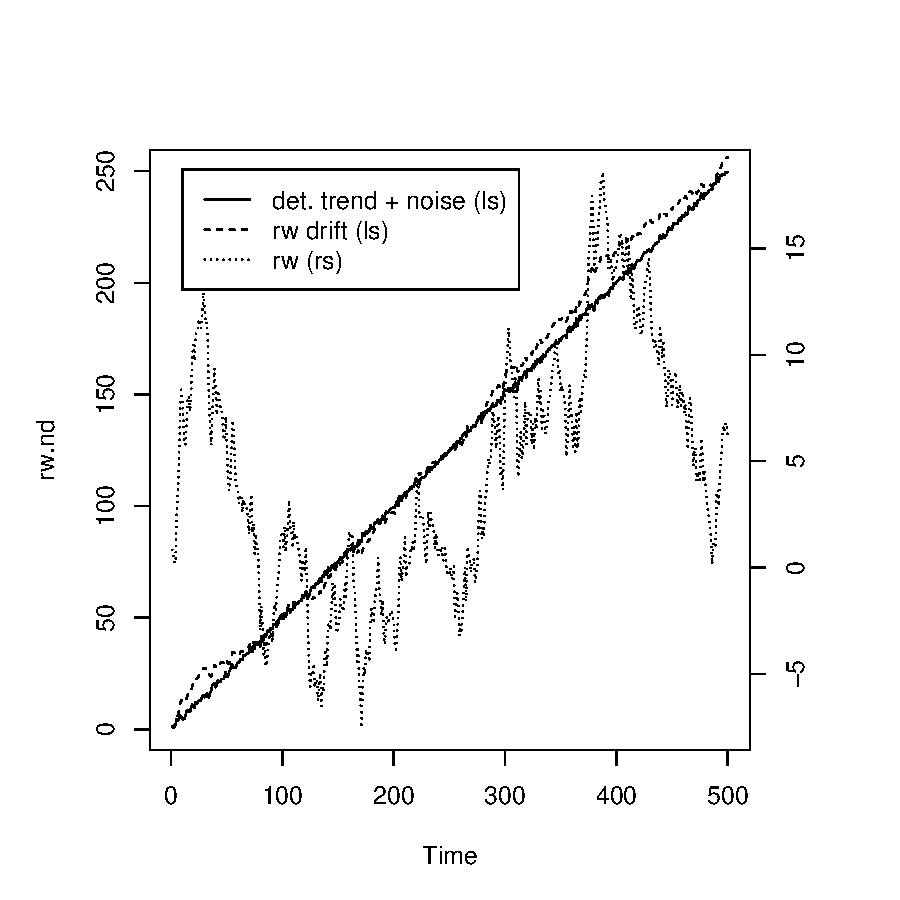
\includegraphics[width=\maxwidth]{figure/plotting} 

\end{knitrout}

There are also a series of tests that can be put in place to assess the nature of the time series.  There are three types of stationary series: \emph{trend stationary}, \emph{difference stationary} and \emph{difference stationary with a constant}

The following equation can be estimated with \emph{Information Criteria} used to assess the appropriate lags of the dependent variable to introduce to remove any serial correlation in the residuals. 
\begin{equation}
\Delta y_t = \beta_1 + \beta_2 t + \pi y_{t-1} +\sum_{j=1}^k \gamma_j \Delta y_i + u_{1t}
\end{equation}

\begin{knitrout}
\definecolor{shadecolor}{rgb}{0.969, 0.969, 0.969}\color{fgcolor}\begin{kframe}
\begin{alltt}
\hlfunctioncall{library}(urca)
\hlfunctioncall{library}(xtable)
\hlfunctioncall{data}(Raotbl3)
\hlfunctioncall{attach}(Raotbl3)
lc <- \hlfunctioncall{ts}(lc, start = \hlfunctioncall{c}(1966, 4), end = \hlfunctioncall{c}(1991, 2), frequency = 4)
lc.ct <- \hlfunctioncall{ur.df}(lc, lags = 3, type = \hlstring{"trend"})
\hlfunctioncall{print}(\hlfunctioncall{xtable}(\hlfunctioncall{summary}(lc.ct)))
\end{alltt}


{\ttfamily\noindent\bfseries\color{errorcolor}{\#\# Error: no applicable method for 'xtable' applied to an object of class "sumurca"}}\end{kframe}
\end{knitrout}


%lc.co <- ur.df(lc, lags=3, type='drift')
%lc2 <- diff(lc)
%lc2.ct <- ur.df(lc2, type='trend', lags=3)
%@




\section{Cointegration}
This is the overview of conintegration and the methods use to analyse conintegrated relationships. Non-stationary data may exhibit \emph{spurious regression}.  If two norman random variables are created (e1 and e2) and two series (y1 and y2) have a trend plus a random shock. 
\begin{knitrout}
\definecolor{shadecolor}{rgb}{0.969, 0.969, 0.969}\color{fgcolor}\begin{kframe}
\begin{alltt}
\hlfunctioncall{library}(lmtest)
\hlfunctioncall{library}(xtable)
\hlfunctioncall{set.seed}(123456)
e1 <- \hlfunctioncall{rnorm}(500)
e2 <- \hlfunctioncall{rnorm}(500)
trd <- 1:500
y1 <- 0.8 * trd + \hlfunctioncall{cumsum}(e1)
y2 <- 0.6 * trd + \hlfunctioncall{cumsum}(e2)
\end{alltt}
\end{kframe}
\end{knitrout}

Now plot the two series
\begin{knitrout}
\definecolor{shadecolor}{rgb}{0.969, 0.969, 0.969}\color{fgcolor}\begin{kframe}
\begin{alltt}
\hlfunctioncall{plot}(y1, type = \hlstring{"l"}, main = \hlstring{"Plot of y1 and y2"}, col = \hlstring{"red"}, ylab = \hlstring{"y1, y2"})
\hlfunctioncall{lines}(y2, col = \hlstring{"blue"})
\end{alltt}
\end{kframe}
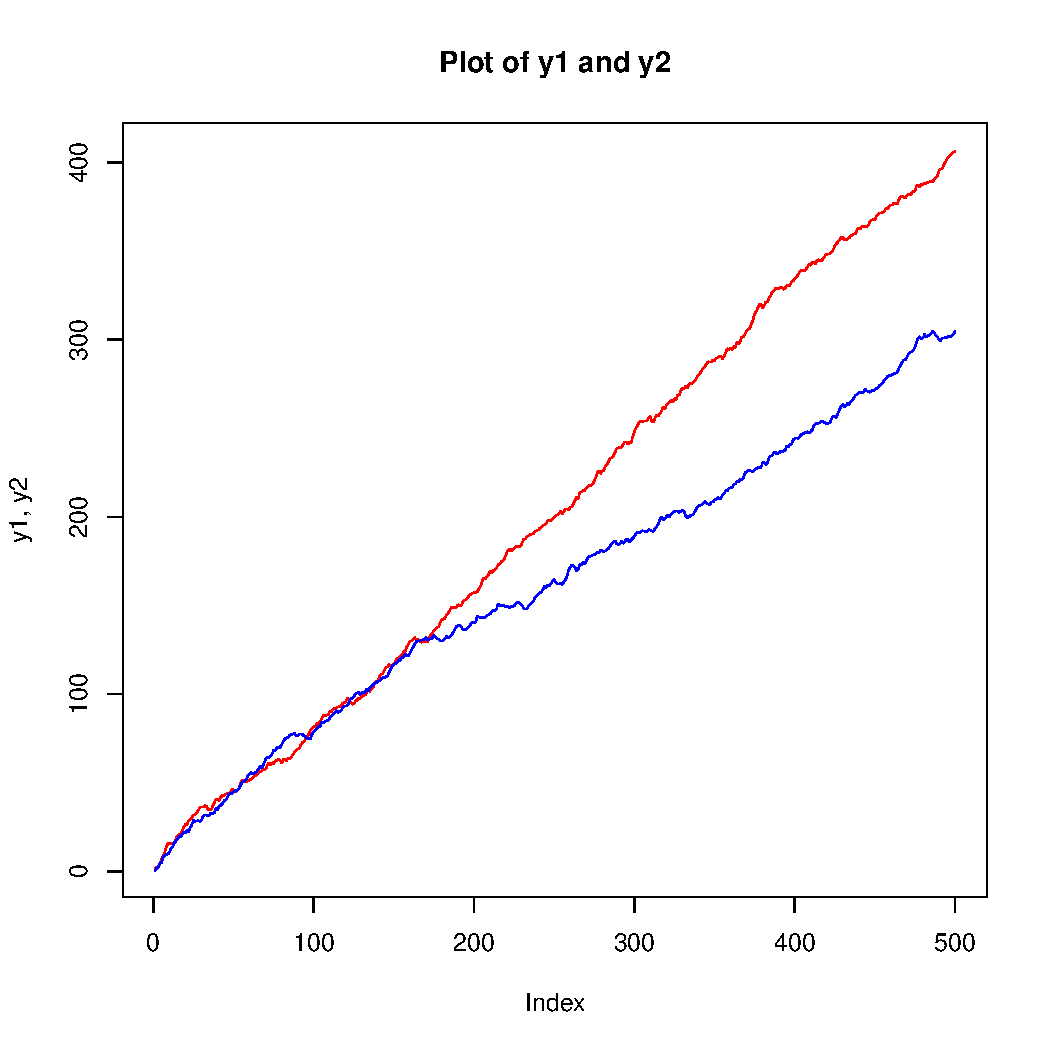
\includegraphics[width=\maxwidth]{figure/plot} 

\end{knitrout}

Run a regression of $y1$ on $y2$ and it appears that there is a strong relationship.  
\begin{kframe}
\begin{alltt}
sr.reg <- \hlfunctioncall{lm}(y1 ~ y2)
\hlfunctioncall{print}(\hlfunctioncall{xtable}(sr.reg))
\end{alltt}
\end{kframe}% latex table generated in R 2.15.2 by xtable 1.7-0 package
% Tue Jun 04 21:47:54 2013
\begin{table}[ht]
\begin{center}
\begin{tabular}{rrrrr}
  \hline
 & Estimate & Std. Error & t value & Pr($>$$|$t$|$) \\ 
  \hline
(Intercept) & -29.3270 & 1.3672 & -21.45 & 0.0000 \\ 
  y2 & 1.4408 & 0.0075 & 191.62 & 0.0000 \\ 
   \hline
\end{tabular}
\end{center}
\end{table}


However, the Durbin-Watson statistics shows there is a large amount of auto-correlation in the residuals.  
\begin{knitrout}
\definecolor{shadecolor}{rgb}{0.969, 0.969, 0.969}\color{fgcolor}\begin{kframe}
\begin{alltt}
sr.dw <- \hlfunctioncall{dwtest}(sr.reg)$statistic
sr.dw
\end{alltt}
\begin{verbatim}
##      DW 
## 0.01715
\end{verbatim}
\end{kframe}
\end{knitrout}

The statistic will be around 2 if there is no autocorrelation. 
\end{document}
